This chapter starts looking at the case where the MDP models are
large. In the current chapter we will look at approximating the
value function. In the next chapter we will consider learning
directly a policy and optimizing it.

When we talk about a large MDP, it can be in one of a few different
reasons. The most common is having a large state space. For example,
Backgammon has $10^{20}$ states, Go has $10^{170}$ and robot control
has continuous state space. Another dimension is the action space,
which can be even continuous in many applications (say, robots).
Finally, we might have a complex dynamics which are hard to describe
succinctly. The main challenge is that we need our algorithm to
scale up to this enormous spaces.

 Previously, we had a look-up table for the value
function $\Value^\policy(\state)$ or $Q^\policy(\state,\action)$,
which we updated every time we encountered the state $\state$.
%
Here, we will consider function approximation for large MDPs, mainly
large state spaces.
%
In a large state space this will be infeasible. Not only that we do
not have the memory, but even more importantly, we are unlikely to
observe states re-occurring. We will need to make (implicit)
assumptions about the MDP, which can be viewed similarly to our
assumption in learning a classifier in supervised learning.

Specifically, we will have the value functions parameterized by {\em
weights} $\weight$, namely, $\widehat{V}(\state;\weight)\approx
\Value^\policy(\state)$ and
$\widehat{Q}(\state,\action;\weight)\approx
Q^\policy(\state,\action)$. We would like to guarantee
generalization from the observed states and trajectories to
unobserved states and trajectories. In the process we will update
the weights $\weight$, using some learning procedure, most notably
using MC or TD learning.

When considering a value function there are a few interpretations
what exactly we mean. It can either be: (1) mapping from a state
$\state$ to its expected return, i.e.,
$\widehat{V}^\policy(\state;\weight)$. (2) mapping from state-action
pairs $(\state,\action)$ to their expected return, i.e.,
$\widehat{Q}^\policy(\state,\action;\weight)$. (3) mapping from
states $\state$ to expected return of each action, i.e.,
$\langle\widehat{Q}^\policy(\state,\action_i;\weight):\action_i\in
\Actions\rangle$. All the interpretations are valid, and our
discussion will not distinguish between them. (Actually, for
$\langle\widehat{Q}^\policy(\state,\action_i;\weight):\action_i\in
\Actions\rangle$ we implicitly assume that the number of actions is
small.)

We now need to discuss how will we build the approximating function.
For this we can turn to the rich literature in Machine Learning and
consider popular hypothesis classes. For example: (1) Linear
functions, (2) Neural networks, (3) Decision trees, (4) Nearest
neighbors, (5) Fourier or wavelet basis, etc. We will concentrate
here on linear functions and neural networks, mainly since gradient
based methods apply to them very naturally.

We will consider in this chapter (mainly) the discounted return with
a discount parameter $\gamma\in(0,1)$. The results extend very
naturally to the finite horizon and episodic settings.

\textbf{YM: Maybe better to switch to finite horizon, and avoid the
need for mixing time and stead state distribution?}

\section{Basic Approximation}

Before we start the discussion on the learning methods, we will do a
small detour. We will discuss the effect of having an error in the
value function we learn, and its effect on the outcome. Assume we
have a value function $V$ such that $\|V-\Value^*\|_\infty\leq
\varepsilon$. Let $\policy$ be the greedy policy with respect to
$V$, namely,
\[
\policy(\state)=\arg\max_\action [\reward(\state,\action)+\gamma
E_{\state'\sim p(\cdot|\state,\action)}[V(\state')]
\]


\begin{theorem}
Let $V$ such that $\|V-\Value^*\|_\infty\leq \varepsilon$ and
$\policy$ be the greedy policy with respect to $V$. Then,
\[
\|\Value^\policy-\Value^*\|_\infty\leq\frac{2\gamma\varepsilon}{1-\gamma}
\]
\end{theorem}

\begin{proof}
Consider two operators $\operator^\policy$ and $\operator^*$ (see
Chapter \ref{ss:DP_op}). The first $\operator^\policy$ is
\[
(\operator^\policy v)(\state)=\reward(\state,\policy(\state))+\gamma
E_{\state'\sim p(\cdot|\state,\policy(\state))}[v(\state')],
\]
and it converges to $\Value^\policy$ (see Theorem~\ref{thm:DP_op}).


The second $T^*$ is
\[
(\operator^* v)(\state)=\max_\action[\reward(\state,\action)+\gamma
E_{\state'\sim p(\cdot|\state,\action)}[v(\state')] ],
\]
and it converges to $\Value^*$ (see Theorem~\ref{thm:DP_op}).

In addition, recall that we have showed that both
$\operator^\policy$ and $\operator^*$ are $\gamma$-contracting (see
Theorem~\ref{thm:DP_op}).

Since $\policy$ is greedy with respect to $V$ we have
$\operator^\policy V=\operator^* V$ (but this does not hold for
other value functions $V'$).

Then,
\begin{align*}
\|\Value^\policy-\Value^*\|_\infty &= \|T^\policy \Value^\policy - \Value^*\|_\infty\\
&\leq \|T^\policy \Value^\policy -T^\policy V\|_\infty +\|T^\policy V - \Value^*\|_\infty\\
&\leq \gamma\| \Value^\policy - V\|_\infty +\|T^* V - T^*\Value^*\|_\infty\\
&\leq \gamma\| \Value^\policy - V\|_\infty +\gamma\| V - \Value^*\|_\infty\\
&\leq \gamma(\| \Value^\policy - \Value^*\|_\infty+ \|\Value^*-V\|_\infty ) +\gamma\| V - \Value^*\|_\infty\;,
\end{align*}
where in the second inequality we used the fact that since since
$\policy$ is greedy with respect to $V$ then $T^\policy V=T^* V$.

Reorganizing the inequality and recalling that
$\|\Value^*-\Value\|_\infty\leq \varepsilon$, we have
\[
(1-\gamma)\|\Value^\policy-\Value^*\|_\infty \leq 2\varepsilon\gamma
\]
and the theorem follows.
\end{proof}

The above theorem states that if we have a small errors in
$L_\infty$ norm, the effect of the errors on the expected return is
bounded. However, in most cases we will not be able to guarantee an
approximation in norm $L_\infty$. This is since it is infeasible even
to compute the $L_\infty$ norm of two given value function, since
this requires considering {\em all} states. In the large state space
setting such operations are infeasible.

\section{From RL to ML}

We would like to reduce our reinforcement learning problem to a
supervised learning problem. This will enable us to use any of the
many techniques of machine learning to address the problem. Let us
consider the basic ingredients of supervised learning. The most
important ingredient is having a labeled sample set, which is
sampled i.i.d.

Let us start by considering an idealized setting. Fix a policy
$\policy$ that we like to learn its value function. We like to
generate a sample
\[
\{(\state_1, \Value^\policy(\state_1)),\ldots,
(\state_m,\Value^\policy(\state_m))\}
\]
We first need to discuss how to sample the states $\state_i$ in an
i.i.d. way. We can generate trajectory, but we need to be careful,
since adjacent states are definitely dependent! One solution is to
space the sampling from the trajectory using the mixing time of
$\policy$.\footnote{See Chapter \ref{chapter:MC} for definition.}
This will give us samples $\state_i$ which are (almost) from the
stationary distribution of $\policy$ and are (almost) independent.
%For the action, we clearly will use $\policy$, no problem there.

The hardest, and most confusing, ingredient is the labels
$\Value^\policy(\state_i)$. In machine leaning we actually assume
that someone gives us the labels to build a classifier.
% (or alternatively, in unsupervised learning, where there is no clear ground truth).
If someone is able to give us
$\Value^\policy(\state)$, it seems like assuming the problem away,
since this is what we would like to learn.

Actually we need to define three things: (1) sample states and actions,
which we will do using $\policy$, (2) a loss function, which will
give the tradeoffs between different approximation errors, and (3)
labels, which we are not given explicitly.

For the state and actions we will define a threshold $\tau$, which
will depends on the mixing time. We will run the policy $\policy$
for $\tau$ steps and then output the state $\state$ (and action
$\action$, if needed).

For the loss function we will define a differential loss function
$J(\weight)$. This will enable us to compute the gradient of the
loss function $\nabla_\weight
J(\weight)=\langle\frac{\partial}{\partial \weight_1}J(\weight),
\ldots , \frac{\partial}{\partial \weight_d}J(\weight)\rangle$, and
update the weights in the negative direction of the gradient,
namely, $\Delta \weight=-\alpha\nabla_\weight J(\weight)$, where
$\alpha$ is the step size of the learning rate. In supervised
learning we are guaranteed that the process will converge to a local
minimum (or a saddle point).

Let us start by defining the loss function,
\[
J(\weight)=\frac{1}{2}\sum_s
\mu(\state)(\Value^\policy(\state)-\widehat{V}^\policy(\state;\weight))^2
\]
where $\mu(\state)$ is the steady state distribution of
$\policy$.\footnote{See Chapter \ref{chapter:MC} for definition.} Given the loss function $J(\weight)$, we can optimize it by Gradient Descent, i.e., compute the gradient and update the weights. The Stochastic
Gradient Descent (SGD) is simply sampling a single state $\state$
and using it to update, i.e.,
\[
\Delta \weight_\ttime = \alpha (\Value^\policy
(\state)-\widehat{V}^\policy(\state;\weight))\nabla
\widehat{V}^\policy (\state;\weight)
\]

We now need to build the sample, namely, how do we set the labels to
replace $\Value^\policy (\state)$. The basic idea is to find an
unbiased estimator $U_\ttime$ such that $E[U_\ttime
|\state_\ttime]=\Value^\policy(\state_\ttime)$. We now will present
a few different approaches to derive such unbiased estimators.

The simplest approach is to use Monte-Carlo (MC)
sampling.\footnote{See Chapter \ref{sec:MC}} Recall that in First
Visit Monte-Carlo we have $R_\ttime(\state)=\sum_{\tau=1}^T
\reward_\tau$, starting at the first visit of $\state$ in episode
$\ttime$. Clearly, we have
$E[R_\ttime(\state)]=\Value^\policy(\state)$, since samples are
independent, so we can set $U_\ttime(\state)=R_\ttime(\state)$. The
update becomes,
\[
\Delta \weight_\ttime = \alpha
(R_\ttime(\state)-\widehat{V}^\policy(\state;\weight_\ttime))\nabla_{w}
\widehat{V}^\policy (\state;\weight)
\]

We can try to use the same idea for $TD(0)$.\footnote{See Chapter
\ref{sec:TD}.} The estimate of $TD(0)$ for $\state_\ttime$ is
$R_\ttime(\state_\ttime)=\reward_\ttime+\gamma
\widehat{V}^\policy(\state_{\ttime+1};\weight)$. The first problem
is that this is a biased estimator since
\[
\Value^\policy(\state_\ttime)=E[\reward_\ttime+\gamma
\Value^\policy(\state_{\ttime+1})]\neq E[\reward_\ttime+\gamma
\widehat{V}(\state_{\ttime+1};\weight)]\;.
\]
We have an additional problem with the gradient, since we have
$\weight$ influencing also the target $R_\ttime(\state_\ttime)$
through $\widehat{V}^\policy(\state_{\ttime+1};\weight)$, something
we do not have in MC (or generally in ML). For this reason
$\nabla_\weight \widehat{V}(\state_\ttime;\weight)$ is called a
semi-gradient. The update becomes,
\[
\Delta \weight (\state)= \alpha[\reward_\ttime +\gamma
\widehat{V}(\state_{\ttime+1};\weight)-\widehat{V}(\state_\ttime)]\nabla_\weight
\widehat{V}(\state_\ttime;\weight)
\]

Finally we get to $TD(\lambda)$. Similar to $TD(0)$ we can now
define the forward update to be,
\[
\Delta \weight =  \alpha[R^\lambda_\ttime
-\widehat{V}(\state_\ttime;\weight)]\nabla_\weight
\widehat{V}(\state_\ttime;\weight)
\]
and the backward update,
\begin{align*}
e_\ttime &= \gamma\lambda e_{\ttime-1}+\nabla_\weight \widehat{V}(\state_\ttime;\weight)\\
\Delta_\ttime &= \reward_\ttime+\gamma \widehat{V}(\state_{\ttime+1};\weight)-\widehat{V}(\state_{t};\weight)\\
\Delta \weight &= \alpha \Delta_\ttime e_\ttime
\end{align*}


\section{Linear Functions}

We first start with the state encoding. In general we assume that
each state $\state$ is encoded by a vector $x(\state)\in
\mathbb{R}^d$. For notation, let $x(\state)=(x_1(\state),\ldots ,
x_d(\state))$. This will be useful for any hypothesis, and
specifically, linear function and neural networks.

A linear function is characterized by a vector of weights
$\weight\in \mathbb{R}^d$. The value of the function at state
$\state$ is
\[
\widehat{V}(\state;\weight)=\weight^\top x(\state)
\]
This implies that the SGD updates become
\[
\weight_{\ttime+1}=\weight_\ttime \alpha[U_\ttime
-\widehat{V}(\state_\ttime;\weight_\ttime)]x(\state_\ttime)
\]

The main benefit of the linear function is when $d\ll |\States|$.
When $d=|\States|$ we can simply encode a look-up table using
$\weight$. This is done by setting the encoding of each state to be
the unit vector $x_i(\state)=I(\state=\state_i)$, and the
approximation to be $\widehat{V}(\state;\weight)=\sum_{i=1}^d
\weight_i I(\state=\state_i)$. This implies that
$\widehat{V}(\state_i;\weight)=\weight_i$.

For a linear function the gradient is simply $x(\state)$, i.e.,
$\nabla_\weight \weight^\top x(\state)=x(\state)$. The Monte-Carlo
update will become
\[
\Delta \weight=
\alpha[R_\ttime-\widehat{V}(\state_\ttime;\weight_\ttime)]x(\state_\ttime)
\]
For $TD(0)$ we have
\[
\Delta \weight= \alpha[\reward_\ttime+\gamma
\widehat{V}(\state_{\ttime+1};\weight_\ttime)-\widehat{V}(\state_\ttime;\weight_\ttime)]x(\state_\ttime)
\]
For $TD(\lambda)$, for the forward view we have
\[
\Delta \weight=
\alpha[R^\lambda_\ttime-\widehat{V}(\state_\ttime;\weight_\ttime)]x(\state_\ttime)
\]
For the backward view we have,
\begin{align*}
e_\ttime &= \gamma\lambda e_{\ttime-1}+x(\state_\ttime)\\
\Delta_\ttime &= \reward_\ttime+\gamma \widehat{V}(\state_{\ttime+1};\weight_\ttime)-\widehat{V}(\state_{t};\weight_\ttime)\\
\Delta \weight &= \alpha \Delta_\ttime e_\ttime
\end{align*}

%\paragraph{Monte-Carlo:}

We would like to discuss the convergence of the different
algorithms. Recall that the mean squared error loss function is
strongly convex, i.e.,
\[
J(\weight)=\frac{1}{2}\sum_{\state\in\States}
\mu(\state)(\Value^\policy(\state)-\widehat{V}^\policy(\state;\weight))^2\;.
\]
Therefore there is a unique $\weight_{min}$ which minimizes
$J(\weight)$. Monte-Carlo is simply running a Stochastic Gradient
Decent (SGD) algorithm, and therefore the convergence and its rate
follow from known results in convex optimization.

The convergence of $TD$ is more problematic, since it uses a
semi-gradient and not the true gradient. The good news is that for
linear functions, when using an on-policy, there is a proof of
convergence. However, the convergence is not to $\weight_{min}$ but
rather to a different point $\weight_{TD}$. The difference is due to
the fact that we are minimizing the expression
\[
\weight_{TD}=\arg\min_\weight\frac{1}{2}\sum_s
\mu(\state)\left(\reward(\state,\policy(\state))+\gamma
E_{\state'}[\widehat{V}(\state';\weight_\ttime)]-\widehat{V}^\policy(\state;\weight)\right)^2
\]
The difference in the losses can be bounded as follows\footnote{ The
derivation appears in Section \ref{sec:FA-Advanced}.}
\[
J(\weight_{TD})\leq \frac{1}{1-\gamma}J(\weight_{min})
\]
Note that for $\gamma\approx 1$, which is a popular setting, we
might have a huge multiplicative factor, yet bounded. However, if we
are in the realizable case, $J(\weight_{min})=0$, then we have also
$J(\weight_{TD})=0$.




\section{Off-policy}
\label{sec:TD-FA}

We would like to see what is the effect that the samples come when
following a different policy, namely, an off-policy setting. There
is no issue for Monte-Carlo, and the same logic would still be
valid.  For TD, we did not have any problem in the look-up model. We
would like to see what can go wrong when we have a function
approximation setting.


\begin{figure}
  % Requires \usepackage{graphicx}
  \begin{centering}
  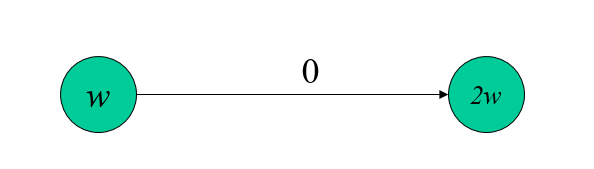
\includegraphics[width=0.5\textwidth]{figures/L8-2states.png}\\
  \caption{Two state snippet of an MDP }\label{fig:L8-2state}
  \end{centering}
\end{figure}

Consider the following part of an MDP (see Figure
\ref{fig:L8-2state}) consists of two nodes, with a transition from
the first to the second, with reward $0$. The main issue is that the
linear approximation gives the first node a weight $\weight$ and the
second $2\weight$. Assume we start with some value $\weight_0>0$.
Each time we have an update for the two states we have
\[
\weight_{\ttime+1}=\weight_\ttime +\alpha[0+\gamma
(2\weight_\ttime)-\weight_\ttime]=[1+\alpha(2\gamma-1)]\weight_\ttime=[1+\alpha(2\gamma-1)]^\ttime\weight_1
\]
For $\gamma>0.5$ we have $\alpha(2\gamma-1)>0$, and $\weight_\ttime$
diverges.

We are implicitly assuming that the setting is off-policy, since in
an on-policy, we would continue from the second state, and
eventually lower the weight.

To have a ``complete'' example consider the three state MDP in
Figure~\ref{fig:L8-3state}. All the rewards are zero, and the main
difference is that we have a new terminating state, that we reach
with probability $p$.

\begin{figure}
  % Requires \usepackage{graphicx}
  \begin{centering}
  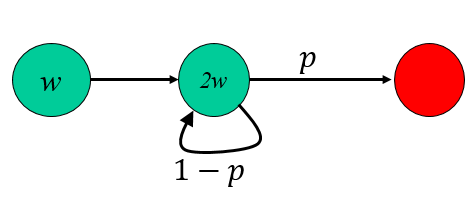
\includegraphics[width=0.5\textwidth]{figures/L8-3state.png}\\
  \caption{The three state MDP. All rewards are zero.}\label{fig:L8-3state}
  \end{centering}
\end{figure}




Again, assume that we start with some $\weight_0>0$ We have three
types of updates, one per possible transition. When we transition
from the initial state to the second state we have
\[
\Delta \weight= \alpha[0+\gamma
(2\weight_\ttime)-\weight_\ttime]\cdot
1=\alpha(2\gamma-1)\weight_\ttime
\]
The transition from the second state back to itself has an update,
\[
\Delta \weight= \alpha[0+\gamma
(2\weight_\ttime)-(2\weight_\ttime)]\cdot 2
=-4\alpha(1-\gamma)\weight_\ttime
\]
The transition to the terminal state we have
\[
\Delta \weight= \alpha[0+\gamma 0 -(2\weight_\ttime)]\cdot
2=-4\alpha \weight_\ttime
\]



When we use on-policy, we have all transitions. Assume that the
second transition happens $n\geq 0$ times. Then we have
\[
\frac{\weight_{\ttime+1}}{\weight_\ttime}=(1+\alpha(2\gamma-1))(1-4\alpha(1-\gamma))^n(1-4\alpha)<
1-\alpha
\]
This implies that $\weight_\ttime$ converges to zero, as desired.

Now consider an off-policy that truncates the episodes after $n$
transitions of the second state, where $n\ll 1/p$, and in addition
$\gamma> 1-1/(40n)$. This implies that in most updates we do not
reach the terminal state and we have
\[
\frac{\weight_{\ttime+1}}{\weight_\ttime}=(1+\alpha(2\gamma-1))(1-4\alpha(1-\gamma))^n>1
\]
and therefore, for the some setting of $n$ we have that the weight
$\weight_\ttime$ diverges.

We might hope that the divergence is due to the online nature of the
TD updates. We can consider an algorithm that in each iteration
minimizes the square error. Namely,
\[
\weight_{\ttime+1}=\arg\min_\weight\sum_s
[\widehat{V}(\state_\ttime;\weight)-E^\policy[\reward_\ttime+\gamma\widehat{V}(\state_{\ttime+1};\weight_\ttime)]]^2
\]

For the MDP example of Figure~\ref{fig:L8-3state} we have that:
\begin{align*}
 \weight_{\ttime+1} &= \arg\min_\weight (\weight-\gamma(2\weight_\ttime))^2+(2\weight-(1-p)\gamma(2\weight_\ttime))^2
\end{align*}
Solving for $\weight_{\ttime+1}$ we have
\begin{align*}
0&=  2(\weight_{\ttime+1}-\gamma(2\weight_\ttime))+4(2\weight_{\ttime+1}-(1-p)\gamma(2\weight_\ttime)\\
  10 \weight_{\ttime+1}&=4\gamma \weight_\ttime + 8\gamma(1-p)\weight_\ttime\\
  \weight_{\ttime+1}&=\frac{6-4p}{5}\gamma \weight_\ttime
\end{align*}
So for $\gamma(6-4p)>5$ we have divergence. (Recall that
$\gamma\approx 1-\varepsilon$ and $p\approx \varepsilon$ is a very
important setting.)

Note that if we have taken in to account the influence of
$\weight_{\ttime+1}$ on $V$ and use
$\widehat{V}(\state_{\ttime+1};\weight_{\ttime+1})$ instead of
$\widehat{V}(\state_{\ttime+1};\weight_\ttime)$, this specific
problem would have disappeared, since $\weight_{\ttime+1}=0$ would
be the minimizer.

\section{Summary}

What we have seen, as Rich Sutton says, that there is a {\em deadly
triad}:
\begin{enumerate}
\item
Function Approximation
\item
Bootstrapping methods, such as TD.
\item
Off-policy training.
\end{enumerate}
When the three conditions hold, many times we have counter examples for the convergence.

Here is a summary of the known convergence and divergence results in
the literature:
\begin{center}
  \begin{tabular}{ | l | c | c|c|c| }
    \hline
    & algorithm & look-up table&linear function&non-linear\\ \hline
    on-policy & MC & + & + & + \\ \hline
    on-policy & $TD(0),TD(\lambda)$ & + & + & -\\ \hline
 %   on-policy & $TD(\lambda)$ & + & + & - \\ \hline
    off-policy & MC & + & + & + \\ \hline
    off-policy & $TD(0),TD(\lambda)$ & + & - & -\\ \hline
 %   off-policy & $TD(\lambda)$ & + & - & - \\ \hline
  \end{tabular}
\end{center}

The results for the look-up table where derived in Chapter
\ref{chapter:learning-model-free}.
%
The fact that Monte-Carlo methods converge is due to the fact that
they are running an SGD algorithm. For linear functions with convex
loss they will converge to the global optimum and for non-linear
functions (for example, neural networks) they will converge to a
local optima. The convergence to the TD appear in Chapter
\ref{sec:FA-Advanced}. The divergence of TD with linear fucntions in
an off-policy setting appear in Chapter \ref{sec:TD-FA}. The TD
divergence in the non-linear online setting appears in
\cite{TsitsiklisVR97}.


%\newpage
\begin{leftbar}
\section{Advanced topics}
\label{sec:FA-Advanced}

\subsection{Comparing $\weight_{min}$ and $\weight_{TD}$}

The derivation follows \cite{TsitsiklisVR97}, however, for
simplicity, we limit ourselves to $TD(0)$ rather than $TD(\lambda)$.

We will need to start with a few definitions. Given the steady state
distribution $\mu(\state)$ for $\state\in \States$ we define a
diagonal matrix $D$ of size $|\States|\times|\States|$ where
$D(\state,\state)=\mu(\state)$. We define an inner-product
$\langle\cdot,\cdot\rangle_D$ where $\langle
z_1,z_2\rangle_D=z_1^\top Dz_2$ and a norm $\|z\|_D=\sqrt{<z,z>_D}$.

We define $\operator^\policy(V)= \reward + \gamma PV$ and recall
that: (1) $\Value^\policy = \operator^\policy(\Value^\policy)$, (2)
$\|\operator^\policy(V_1)-\operator^\policy(V_2)\|_D\leq \gamma
\|V_1-V_2\|_D$ (actually we we need to prove that for
$\|\cdot\|_D$).

We will perform a linear function approximation where the attributes
of state $\state$ are $x_\state$. Define a matrix $X$ of size
$|\States|\times d$, where the $\state$ row is $x_\state$. Then
using a parameter $\weight$ our approximation is
$\widehat{V}(\cdot;\weight)=X\weight$. We now need to project
vectors to an approximation $X\weight$. Give a vector $V$, let
$\Pi(V)=\arg\min_\weight \|X\weight-V\|_D$. This projection
operation can be written explicitly as
\[
\Pi(V)=X(X^\top DX)^{-1}X^\top D V.
\]


We can write the expected update as:
\[
\Delta \weight= X^\top D(T^\policy(X\weight_\ttime)-X\weight)
\]
which is the gradient of
\[
\nabla_\weight \|T^\policy(X\weight_\ttime)-Xw\|_D^2
\]
note that the input to $T^\policy$ is fixed and we optimize over
$\weight$ only. The minimization is
\[
\weight_{\ttime+1}=\Pi(T^\policy(X\weight_\ttime))
\]

We will need the following technical claim:
\begin{claim}
\[
\|PV\|_D^2\leq \|V\|_D^2
\]
\end{claim}

\begin{proof}
\begin{align*}
\|PV\|_D^2 & =V^\top P^\top D P V \\
&= \sum_s \mu(\state) (\sum_{\state'} p(\state'|\state) V(\state'))^2\\
&\leq \sum_s \mu(\state) \sum_{\state'} p(\state'|\state) V^2(\state')\\
&=\sum_{\state'} V^2(\state') \sum_s \mu(\state)p(\state'|\state)\\
&=\sum_{\state'} \mu(\state')V^2(\state')=\|V\|_D
\end{align*}
\end{proof}

\begin{lemma}
Let $\weight_{TD}$ be the limit of
$\weight_{\ttime+1}=\Pi(T^\policy(X\weight_\ttime))$, i.e., using
$TD(0)$. Then,
\[
\|X\weight_{TD}-\Value^\policy\|_D\leq
\frac{1}{1-\gamma}\|X\weight_{min}-\Value^\policy\|_D
\]
\end{lemma}

\begin{proof}
By definition, $\weight_{min}$ is the projection of $\Value^\policy$
to $X$, i.e., $\Pi(\Value^\policy)$. Note that we have
$\Value^\policy=
\Pi(\Value^\policy)+(\Value^\policy-\Pi(\Value^\policy))$ and
$\langle\Pi(\Value^\policy),\Value^\policy-\Pi(\Value^\policy)\rangle_D=0$,
otherwise we can improve. This implies that
$\|\Value^\policy\|_D=\|\Pi(\Value^\policy)\|_D+\|\Value^\policy-\Pi(\Value^\policy)\|_D$.
\begin{align*}
\|X\weight_{TD}-\Value^\policy\| &\leq
\|X\weight_{TD}-\Pi(\Value^\policy\|_D+\|\Pi(\Value^\policy)-\Value^\policy\|_D\\
&= \|\Pi(T^\policy(X\weight_{TD}))-\Pi(\Value^\policy)\|_D+\|\Pi(\Value^\policy)-\Value^\policy\|_D\\
&\leq \|T^\policy(X\weight_{TD})-\Value^\policy\|_D+\|\Pi(\Value^\policy)-\Value^\policy\|_D\\
&\leq \gamma \|X\weight_{TD}-\Value^\policy\|_D+\|\Pi(\Value^\policy)-\Value^\policy\|_D\\
\end{align*}
and the lemma follows since $\Pi(\Value^\policy)=X\weight_{min}$ by
definition of $\weight_{min}$.
\end{proof}


\subsection{LSTD}


We consider least Squares Temporal Difference (LSTD). We will
analyze $LSTD(0)$.

Let $x_\ttime=x_{\state_\ttime}$. The weights:
\begin{align*}
\weight_{\ttime+1} &= \weight_\ttime +\alpha (\reward_\ttime+\gamma
\weight_\ttime^\top x_{\ttime+1}-\weight_\ttime^\top
x_\ttime)x_\ttime\\
\weight_{\ttime+1} &= \weight_\ttime +\alpha (\reward_\ttime
x_\ttime-x_\ttime(x_\ttime-\gamma x_{\ttime+1})^\top \weight_\ttime)
\end{align*}

We have that
\[
E[\weight_{\ttime+1}|\weight_\ttime]=\weight_\ttime +\alpha
(b-A\weight_\ttime)
\]
where $b=E[\reward_\ttime x_\ttime]\in \Reals^d$ and
$A=E[x_\ttime(x_\ttime-\gamma x_{\ttime+1})^\top]\in\Reals^{d\times
d}$.

At convergence we have $\weight=A^{-1}b$.

\end{leftbar}


\section{Applications: games}

\subsection{Backgammon}

Tesauro developed the TD-gammon in the late 1980's and 1990's. The
system uses a neural network approximation, using a $TD(\lambda)$
updates. The initial system was able to win against other computer
programs, which where hand-designed, and later matched the
performance of the best human. For the training the system used
self-play, namely playing against itself.

The neural network has a single hidden layer (with $40/80/160$
nodes, in the three different generations of the project). There are
$198$ inputs. The hidden layer has sigmoidal nodes with
$\sigma(z)=\frac{1}{1+e^{-z}}$. The output $y$ can be viewed as the
probability of winning from a given position.

The $198$ inputs are composed as follows. For each of the $24$ slots
and for each of the two colors, we have four Boolean inputs. The
first indicates if there is a single chip, the second indicates two
or more chips, the third indicates exactly three chips and the
fourth indicates four or more chips. We have two Boolean variables
that indicate who turn it is (one for white and one for black).
Finally, we have two aggregate inputs, per color: (1) number of
chips divided by $2$ and (2) number of chips removed divided by
$15$.

The TD-gammon uses the standard TD updates.
\[
\Delta \weight_\ttime =
\alpha(y_\ttime-y_{\ttime-1})\sum_{k=1}^{t}\lambda^{\ttime-k}\nabla_\weight
y_k
\]
When the game ends we replace $y_\ttime$ by $z$ the outcome of the
game.



The evaluation of the position is done using a max-min tree, whose
depth is $1/2/3$ (depending on the generation). The max-min tree has max layer where the value of
a node is the maximum of their children, and min layer, where the
value of a node is the minimum of their children. Given the tree (of
size at most $20/400/8000$ in different generations) we evaluate the
leaves using the neural network, and propagate the values in the
min-max tree to get the predicted value of a position.

The network is initialized with small random weights. Note that due
to the game nature, even with random policies the game terminates.
The training is done using self-play, where the number of games was
$300K/800K/1500K$ in different generations.

One very intriguing aspect  of the TD-gammon is that it {\em
improved the human performance}. For example, when the first role is
{\tt 4-1}, grandmasters did the $1$ move in location $6$, while the
TD-gammon moved location $24$. Following the TD-gammon, grandmasters
changed their view and started playing those positions in the same
way that TD-gammon did.

\subsection{Attari games}

The system was developed by DeepMind researchers during $2013-2015$.
The system learns to play from the raw video frames, a variety of
$49$ games. The learning uses a neural network and employs
$Q$-learning (and a Deep-Q-Network, DQN).

The neural network works as follows. There is a preprocessing stage
that maps frames of size $210\times 160$ with 128-colors, to
$84\times 84$ and 4-colors. This mapping is fixed and shared by all
games. The neural network has three convolutional layers followed by
one completely connected layer. The output layer has multiple
outputs. The nodes in the network use RelU gates.

The DQN innovations are: (1) Experience reply, reusing the same
example many times, (2) fixed Q-target, when setting the target
update, and (3) clipping the error. To better understand the
innovations, we need to consider the flow of the training.

In the training, we first select an action $\action_\ttime$, using
$\varepsilon$-greedy policy. We observe the reward and the next
state
$(\state_\ttime,\action_\ttime,\reward_\ttime,\state_{\ttime+1})$,
and store them in the reply memory. We sample a mini-batch from the
reply memory. For each sample we use the fixed-Q-target (more
latter). We use the SGD to minimize the MSE.

For the fixed-Q-target, we do the update as follows. We have two
sets of weights $\weight_\ttime$, the current weights, and
$\weight^-_\ttime$ as the fixed weights. We update $\weight_\ttime$
to $\weight^-_\ttime$ every (large) number of plays, setting
$\weight_\ttime=\weight^-_\ttime$. The update at time $\ttime$
becomes:
\[
\Delta \weight_\ttime = \alpha \Gamma_\ttime \nabla_{\weight_\ttime}
Q(\state_\ttime,\action_\ttime;\weight_\ttime)
\]
where
\[
\Gamma_{\ttime}=\reward_\ttime+\gamma \max_\action
Q(\state_{\ttime+1},\action;\weight^-_\ttime)-Q(\state_\ttime,\action_\ttime;\weight_\ttime)
\]
Note that $\weight^-_\ttime$ is used only to estimate the future
return from $\state_{\ttime+1}$. The clipping enforces
$\Gamma_\ttime\in[-1,+1]$.

The system is able to match human performance in $29$ out of $49$
Attari games.







\section{Bibliography Remarks}

The work of Gerald Tesauro on TD-gammon is described in
\cite{Tesauro95,Tesauro02}.

The DeepMind system for playing Attari games is described in
\cite{MnihKSRVBGRFOPB15}.


Part of the outline borrows from David Silver class notes and the
the book of Sutton and Barto \cite{SuttonB98}.
